% title: 从 LaTeX 源文件到可浏览页面
% slug: notes/getting-started
% date: 2026-06-07
% summary: 用一篇示例文章演示这个新网站骨架支持的写法，包括章节、列表、公式、定理块和插图。
% tags: LaTeX, 静态站点, 数学博客

\section{写作方式的变化}

这个站点最关键的改造，是把旧站的“Markdown 为主，数学显示为辅”，切换成“\textbf{LaTeX 为主，HTML 为输出}”。

于是你在内容层面可以继续按照熟悉的方式写：

\begin{enumerate}
\item 小节结构用 `\section`、`\subsection`。
\item 行内公式直接写成 $a_n = \frac{1}{n^2}$。
\item 推导过程可以用 `align` 环境整理。
\item 想强调结论时，可以用 `definition`、`theorem`、`proof` 这一类块。
\end{enumerate}

\subsection{一个短的数学示例}

下面这个例子展示了块级公式环境在页面里的呈现效果：

\begin{align}
\sum_{n=1}^{\infty}\frac{1}{n^2}
&=
\frac{\pi^2}{6}, \\
\sum_{n=1}^{\infty}\frac{1}{n^4}
&=
\frac{\pi^4}{90}.
\end{align}

\begin{theorem}[一个非常基础的结论]
若数列 $(a_n)$ 单调递增且有上界，则 $(a_n)$ 收敛。
\end{theorem}

\begin{proof}
这是实分析中的单调有界定理。证明思路是：取集合 $\{a_n : n \in \mathbb{N}\}$ 的上确界，记作 $L$，再利用上确界定义验证 $a_n \to L$。
\end{proof}

\subsection{图像与版式}

这一版也支持把内容资源放在 `PostCode` 下，然后通过 LaTeX 引入：

\begin{figure}
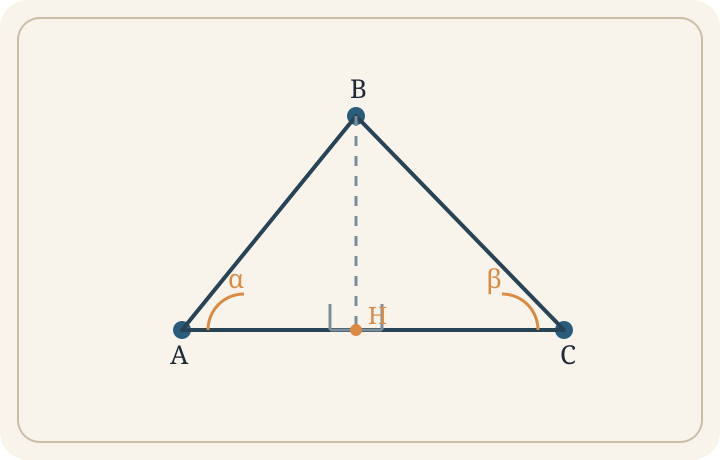
\includegraphics[width=0.72\textwidth]{assets/sample-geometry.svg}
\caption{一个简单的几何示意图，说明图片资源可以和 LaTeX 正文一起组织。}
\end{figure}

\subsection{你后面怎么继续写}

\begin{example}
如果你准备写“高等代数笔记”，可以建立 `PostCode/posts/algebra/`；如果你准备写“实分析习题解析”，可以建立 `PostCode/posts/analysis/`。目录结构本身就会自动反映到左侧文章树里。
\end{example}

如果你想把一篇长文拆成多个文件，也可以把章节拆开后再在主文稿中统一合并，这样大体量文章会更容易维护。
